\documentclass[11pt]{article}
\usepackage[a4paper,margin=27mm]{geometry}
\usepackage[T1]{fontenc}
\usepackage{lmodern,microtype,amsmath,amssymb,amsthm,mathtools,enumitem}
\usepackage{tikz}
\usepackage[colorlinks=true,linkcolor=blue,citecolor=blue,urlcolor=blue]{hyperref}
\hypersetup{pdftitle={Loss Relations for Sets of Desirable Gambles}}

\newtheorem{theorem}{Theorem}[section]
\newtheorem{lemma}[theorem]{Lemma}
\newtheorem{proposition}[theorem]{Proposition}
\newtheorem{corollary}[theorem]{Corollary}
\theoremstyle{definition}
\newtheorem{definition}[theorem]{Definition}
\newtheorem{example}[theorem]{Example}
\newtheorem{remark}[theorem]{Remark}

\newcommand{\R}{\mathbb R}
\newcommand{\one}{\mathbf 1}
\newcommand{\supp}{\operatorname{supp}}
\newcommand{\dH}{d_{\mathrm H}}
\newcommand{\Pc}{\mathcal P}
\newcommand{\Ub}{\overline U}
\newcommand{\Bx}{\operatorname{Box}}
\newcommand{\sd}{\mathbin{\nabla}}
\newcommand{\aev}{\ \text{a.e.}}

\title{Loss Relations for Sets of Desirable Gambles}
\author{}
\date{}

\begin{document}
\maketitle

\section{Setting}\label{sec:setting}

\paragraph{Worlds and gambles.}
Fix $n\ge 2$ and worlds $\omega_1,\dots,\omega_n$. Put $[n]:=\{1,\dots,n\}$ and $S^c:=[n]\setminus S$ for $S\subseteq[n]$. A \emph{gamble} is a vector $g=(g_1,\dots,g_n)\in\R^n$; $g_i$ is its payoff at $\omega_i$. For $g,h\in\R^n$,
\[
g\cdot h:=\sum_{k=1}^n g_kh_k,\qquad \|g\|_1:=\sum_{k=1}^n|g_k|,\qquad \|g\|_\infty:=\max_{k}|g_k|,\qquad \|g\|:=(g\cdot g)^{1/2}.
\]
$g\ge h$ means $g_k\ge h_k$ for all $k$, and $g\gneq 0$ means $g\ge 0$ and $g\neq 0$. $\one:=(1,\dots,1)$, and $e_i$ is the $i$th unit vector.

\paragraph{Probabilities and credal sets.}
$\Delta:=\{p\in\R^n:p\ge 0,\ \sum_kp_k=1\}$, $\supp p:=\{k:p_k>0\}$, and $p(S):=\sum_{k\in S}p_k$ for $S\subseteq[n]$. A \emph{credal set} is a nonempty, closed, convex $K\subseteq\Delta$. For credal sets $K,K'$, $g\in\R^n$ and $i\in[n]$, let
\begin{gather*}
\varphi_K(g):=\min_{m\in K}m\cdot g,\qquad \Ub_K(i):=\max_{m\in K}m_i,\\
\dH(K,K'):=\max\Big\{\max_{m\in K}\min_{m'\in K'}\|m-m'\|_1,\ \max_{m'\in K'}\min_{m\in K}\|m-m'\|_1\Big\}.
\end{gather*}
so $\dH$ is the Hausdorff distance with respect to $\|\cdot\|_1$.

\paragraph{Measure.}
$\mu$ is the standard Gaussian probability measure on $\R^n$:
\[
\mu(Y):=(2\pi)^{-n/2}\int_Ye^{-\|g\|^2/2}\,dg\qquad\text{for Lebesgue measurable }Y\subseteq\R^n.
\]
A set $Y$ is \emph{null} if $\mu(Y)=0$, equivalently if it has Lebesgue measure $0$. Nonempty open sets are not null. $Y\sd Z:=(Y\setminus Z)\cup(Z\setminus Y)$. $Y\subseteq Z$ a.e.\ means $\mu(Y\setminus Z)=0$. $Y\approx Z$ means $\mu(Y\sd Z)=0$.

\paragraph{Models.}
A \emph{model} is a Lebesgue measurable set $X\subseteq\R^n$ (the gambles it accepts). A set $D\subseteq\R^n$ is a \emph{coherent set of desirable gambles} if
\begin{enumerate}[label=(D\arabic*),itemsep=0pt]
\item $0\notin D$;
\item if $g\gneq 0$ then $g\in D$;
\item if $g\in D$ and $\lambda>0$ then $\lambda g\in D$;
\item if $g,h\in D$ then $g+h\in D$.
\end{enumerate}
By (D3) and (D4), a coherent set of desirable gambles is convex, hence Lebesgue measurable (the boundary of a convex set is null). A model $X$ is \emph{coherent} if $X\approx D$ for some coherent set of desirable gambles $D$. For a credal set $K$,
\[
D_K:=\{g:\varphi_K(g)>0\}\cup\{g:g\gneq 0\}.
\]

\paragraph{Errors.}
$G_i:=\{g:g_i>0\}$. The \emph{error set} of a model $X$ at $\omega_i$ is
\[
E_i(X):=X\sd G_i.
\]
For nonempty $T\subseteq[n]$, $G_T^+:=\{g:g_k>0\text{ for all }k\in T\}$ and $G_T^-:=\{g:g_k\le 0\text{ for all }k\in T\}$.

\paragraph{Losses and loss relations.}
A \emph{loss} assigns to each model $X$ and world $\omega_i$ a value $L(X,\omega_i)\in[0,\infty]$. Its \emph{loss relations} are
\[
X\preceq_i Y\ :\iff\ L(X,\omega_i)\le L(Y,\omega_i),\qquad X\prec_i Y\ :\iff\ L(X,\omega_i)<L(Y,\omega_i).
\]
Put $L(X):=(L(X,\omega_1),\dots,L(X,\omega_n))$. $X$ \emph{weakly dominates} $Y$ if $X\preceq_i Y$ for all $i$; $X$ \emph{dominates} $Y$ if moreover $L(X)\neq L(Y)$; $X$ \emph{strictly dominates} $Y$ if $X\prec_i Y$ for all $i$. $Y$ is \emph{undominated} if no model dominates it. For $S\subseteq[n]$, $X$ is \emph{competitive on $S$} if for every model $Y$ some $i\in S$ has $X\preceq_i Y$.

\section{The loss}\label{sec:loss}

A \emph{family} is a map $p\mapsto K_p$ from $\Delta$ to credal sets. Write
\[
\varphi_p:=\varphi_{K_p},\qquad \Ub_p:=\Ub_{K_p},\qquad D_p:=D_{K_p}.
\]
Consider the conditions:
\begin{enumerate}[leftmargin=*,itemsep=2pt]
\item[\textbf{(U)}] For all $p,q\in\Delta$ and $i\in[n]$: if $p_i>q_i$ then $\Ub_p(i)>\Ub_q(i)$.
\item[\textbf{(Lip)}] There is $A\ge 0$ with $\dH(K_p,K_q)\le A\|p-q\|_1$ for all $p,q\in\Delta$.
\item[\textbf{(Dom)}] There is $B\ge 0$ with $\Ub_p(i)\le Bp_i$ for all $p\in\Delta$ and $i\in[n]$.
\end{enumerate}

\begin{definition}\label{def:loss}
For a model $X$ and $i\in[n]$, let
\[
\Pc_i(X):=\{p\in\Delta:E_i(X)\subseteq E_i(D_p)\aev\}.
\]
For $\eta\ge 0$, let
\[
L_\eta(X,\omega_i):=\begin{cases}
\inf\big\{1-p_i-\eta\,\mu\big(E_i(D_p)\setminus E_i(X)\big):p\in\Pc_i(X)\big\} & \text{if }\Pc_i(X)\neq\varnothing,\\[2pt]
2+\mu(E_i(X)) & \text{if }\Pc_i(X)=\varnothing.
\end{cases}
\]
Under (Lip) and (Dom), fix constants $A,B$ as there, and put
\[
\kappa:=8n^2(A+2B),\qquad \eta_0:=\frac{1}{n\kappa}.
\]
(Dom) forces $B\ge1$: for $m\in K_p$, $1=\sum_im_i\le\sum_i\Ub_p(i)\le B$. So $\kappa\ge16n^2>0$. By Theorem~\ref{thm:main}(a), $L_\eta$ is a loss under the hypotheses of that theorem.
\end{definition}

\begin{theorem}\label{thm:main}
Assume (U), (Lip) and (Dom), let $0<\eta<\eta_0$, and let $L:=L_\eta$. Then:
\begin{enumerate}[label=(\alph*)]
\item $L$ takes values in $[0,1]\cup[2,3]$. If $E_i(X)\subseteq E_i(Y)$ a.e., then $X\preceq_iY$; if moreover $\mu(E_i(Y)\setminus E_i(X))>0$, then $X\prec_iY$. If $X\approx Y$, then $L(X)=L(Y)$.
\item $L(D_q,\omega_i)=1-q_i$ for all $q\in\Delta$ and $i\in[n]$.
\item For every $q\in\Delta$, $D_q$ is competitive on $\supp q$.
\item For every model $X$ and $i\in[n]$, the set $\{q\in\Delta:D_q\preceq_iX\}$ is closed.
\item If a model $X$ weakly dominates $D_q$, then $X\approx D_q$. In particular, $D_q$ is undominated.
\item Every model is weakly dominated by some $D_q$. Every model $X$ with $X\not\approx D_p$ for all $p\in\Delta$ is dominated by some $D_q$.
\end{enumerate}
Consequently, the undominated models are exactly the models $X$ with $X\approx D_p$ for some $p\in\Delta$. All of them are coherent.
\end{theorem}

\begin{remark}\label{rem:axioms}
For orientation, in the framework of \cite{KCM}, take every model to be evaluable and the coherent models as in Section~\ref{sec:setting}. By (e) and (f), the coherent undominated models are $\mathcal C_L=\{X:X\approx D_p\text{ for some }p\in\Delta\}$, so (LA) holds. By (b), (c) and (d), $u_p:=D_p$ satisfies (S). By (e), every model with the same loss profile as a member of $\mathcal C_L$ lies in $\mathcal C_L$, which is (C).
\end{remark}

\section{Proofs}\label{sec:proofs}

\begin{lemma}\label{lem:basic}
Let $K,K'$ be credal sets, $g,h\in\R^n$, $t\in\R$, $\lambda\ge 0$ and $i\in[n]$.
\begin{enumerate}[label=(\roman*)]
\item $\varphi_K(g+t\one)=\varphi_K(g)+t$, $\varphi_K(\lambda g)=\lambda\varphi_K(g)$ and $\varphi_K(g+h)\ge\varphi_K(g)+\varphi_K(h)$.
\item $|\varphi_K(g)|\le\|g\|_\infty$, $|\varphi_K(g)-\varphi_K(h)|\le\|g-h\|_\infty$ and $|\varphi_K(g)-\varphi_{K'}(g)|\le\dH(K,K')\|g\|_\infty$.
\item $\varphi_K(\one-\lambda e_i)=1-\lambda\,\Ub_K(i)$.
\item $D_K$ is a coherent set of desirable gambles, and $D_K\approx\{g:\varphi_K(g)>0\}$. If $\varphi_K(g)<0$ then $g\notin D_K$.
\end{enumerate}
\end{lemma}

\begin{proof}
(i) $m\cdot\one=1$ for $m\in\Delta$. The other two hold because a minimum of a sum is at least the sum of the minima.

(ii) For $m\in\Delta$, $|m\cdot g|\le\|m\|_1\|g\|_\infty=\|g\|_\infty$ and $|m\cdot g-m\cdot h|\le\|g-h\|_\infty$; take minima over $m\in K$. For the third claim, pick $m\in K$ with $m\cdot g=\varphi_K(g)$ and $m'\in K'$ with $\|m-m'\|_1\le\dH(K,K')$. Then $\varphi_{K'}(g)\le m'\cdot g\le m\cdot g+\|m'-m\|_1\|g\|_\infty\le\varphi_K(g)+\dH(K,K')\|g\|_\infty$. Exchange $K$ and $K'$.

(iii) $m\cdot(\one-\lambda e_i)=1-\lambda m_i$.

(iv) If $g\gneq 0$ then $\varphi_K(g)\ge 0$. So $\varphi_K\ge 0$ on $D_K$, and $\varphi_K(g)<0$ implies $g\notin D_K$. (D1): $\varphi_K(0)=0$ and $0\not\gneq 0$. (D2): by definition. (D3): by (i), and because $\lambda g\gneq0$ iff $g\gneq0$. (D4): if $g,h\gneq 0$ then $g+h\gneq 0$; otherwise one of $\varphi_K(g),\varphi_K(h)$ is positive and the other is nonnegative, so $\varphi_K(g+h)>0$ by (i). Finally, if $g\in D_K$ and $\varphi_K(g)\le 0$, then $g\gneq 0$ and $m\cdot g=0$ for some $m\in K$, so $g_k=0$ for every $k\in\supp m$. Hence $D_K\setminus\{\varphi_K>0\}\subseteq\bigcup_k\{g:g_k=0\}$, which is null. $D_K$ is a Borel set, since $\{\varphi_K>0\}$ is open by (ii) and $\{g:g\gneq0\}=[0,\infty)^n\setminus\{0\}$.
\end{proof}

\begin{lemma}\label{lem:thin}
For every credal set $K$ and $\delta\ge 0$,
\[
\mu\big(\{g:|\varphi_K(g)|\le\delta\|g\|_\infty\}\big)\le 4n\delta.
\]
Consequently, $\mu(D_K\sd D_{K'})\le 4n\,\dH(K,K')$ for all credal sets $K,K'$.
\end{lemma}

\begin{proof}
If $\delta>\frac12$ the bound exceeds $1$. Let $\delta\le\frac12$. For $g\in\R^n$ put $t:=\frac1n\sum_kg_k$ and $h:=g-t\one$. By Lemma~\ref{lem:basic}, $\varphi_K(g)=\varphi_K(h)+t$ and $|\varphi_K(h)|\le\|h\|_\infty$, so
\[
\|g\|_\infty\le\|h\|_\infty+|t|\le 2\|h\|_\infty+|\varphi_K(h)+t|.
\]
So if $|\varphi_K(g)|\le\delta\|g\|_\infty$, then $(1-\delta)|t+\varphi_K(h)|\le 2\delta\|h\|_\infty$, hence $|t+\varphi_K(h)|\le 4\delta\|h\|_\infty$.

Now let $g$ be a random vector with distribution $\mu$, so $g_1,\dots,g_n$ are independent standard normal. Then $(t,h)$ is jointly normal and $\operatorname{Cov}(t,h_k)=\operatorname{Cov}(t,g_k)-\operatorname{Var}(t)=\frac1n-\frac1n=0$, so $t$ is independent of $h$. Also $t$ is normal with mean $0$ and variance $\frac1n$, so its density is at most $\sqrt{n/(2\pi)}$. Let $I(h):=[-\varphi_K(h)-4\delta\|h\|_\infty,\,-\varphi_K(h)+4\delta\|h\|_\infty]$ and let $\nu$ be the distribution of $t$, so $\nu(I(h))\le8\delta\|h\|_\infty\sqrt{n/(2\pi)}$. By the previous paragraph, $\mu(\{g:|\varphi_K(g)|\le\delta\|g\|_\infty\})\le\Pr(t\in I(h))$, and by independence and Fubini's theorem, $\Pr(t\in I(h))=\mathbb E\,\nu(I(h))$. Since $\mathbb E\|h\|_\infty\le\mathbb E\|h\|\le(\mathbb E\|h\|^2)^{1/2}=\sqrt{n-1}$,
\[
\mu\big(\{g:|\varphi_K(g)|\le\delta\|g\|_\infty\}\big)\le 8\delta\sqrt{n(n-1)/(2\pi)}\le\tfrac{8}{\sqrt{2\pi}}\,n\delta\le 4n\delta.
\]
For the consequence: by Lemma~\ref{lem:basic}(iv), up to a null set $D_K\sd D_{K'}$ consists of $g$ with $\varphi_K(g)>0\ge\varphi_{K'}(g)$ or $\varphi_{K'}(g)>0\ge\varphi_K(g)$. For such $g$, $|\varphi_K(g)|\le|\varphi_K(g)-\varphi_{K'}(g)|\le\dH(K,K')\|g\|_\infty$ by Lemma~\ref{lem:basic}(ii). Apply the bound with $\delta:=\dH(K,K')$.
\end{proof}

\begin{lemma}\label{lem:faces}
Assume (Dom). Let $T\subseteq[n]$ be nonempty and $q\in\Delta$. Then
\[
\mu(G_T^+\setminus D_q)\le 8n^2B\,q(T^c)\qquad\text{and}\qquad\mu(D_q\cap G_T^-)\le 8n^2B\,q(T^c).
\]
\end{lemma}

\begin{proof}
Let $\varepsilon:=B\,q(T^c)$. If $\varepsilon>\frac12$ both bounds exceed $1$. Let $\varepsilon\le\frac12$. For $m\in K_q$, (Dom) gives $m(T^c)\le\sum_{k\in T^c}\Ub_q(k)\le\varepsilon$. So $m(T)\ge 1-\varepsilon$ and $\big|\sum_{k\in T^c}m_kg_k\big|\le\varepsilon\|g\|_\infty$ for every $g$.

Let $g\in G_T^+\setminus D_q$ and $\gamma:=\min_{k\in T}g_k>0$. Then $\varphi_q(g)\le 0$, so $m\cdot g\le0$ for some $m\in K_q$, and
\[
0\ge m\cdot g\ge(1-\varepsilon)\gamma-\varepsilon\|g\|_\infty .
\]
So $\gamma\le\frac{\varepsilon}{1-\varepsilon}\|g\|_\infty\le 2\varepsilon\|g\|_\infty$.

Let $g\in D_q\cap G_T^-$ with $g_k\neq0$ for all $k$ (this excludes a null set), and $\gamma:=\min_{k\in T}|g_k|>0$. Then $g_k<0$ for $k\in T$, so $g\not\gneq0$ and $\varphi_q(g)>0$. Take any $m\in K_q$:
\[
0<m\cdot g\le-(1-\varepsilon)\gamma+\varepsilon\|g\|_\infty .
\]
So $\gamma<2\varepsilon\|g\|_\infty$.

In both cases, up to a null set, $g\in\bigcup_{k\in T}\{g:|g_k|\le 2\varepsilon\|g\|_\infty\}$. Lemma~\ref{lem:thin} with $K=\{e_k\}$, for which $\varphi_K(g)=g_k$, bounds the measure of each of these sets by $8n\varepsilon$. And $|T|\le n$.
\end{proof}

\begin{lemma}\label{lem:twoworlds}
Assume (U). Let $X$ be a model, $i\neq j$, $p\in\Pc_i(X)$ and $q\in\Pc_j(X)$. Then $p_i\le q_i$.
\end{lemma}

\begin{proof}
Let $W:=\{g:g_i<0<g_j\}$. Every $g\in W$ lies outside $G_i$ and inside $G_j$. So for every model $Y$, $E_i(Y)\cap W=Y\cap W$ and $E_j(Y)\cap W=W\setminus Y$. Hence $p\in\Pc_i(X)$ gives $\mu(W\cap X\setminus D_p)=0$, and $q\in\Pc_j(X)$ gives $\mu(W\cap D_q\setminus X)=0$. Therefore
\[
\mu(W\cap D_q\setminus D_p)=0.
\]
Suppose $\Ub_p(i)>\Ub_q(i)$. Then $\Ub_q(i)<1$ and $\Ub_p(i)>0$. Choose $\lambda$ with $\max\{1,1/\Ub_p(i)\}<\lambda<1/\Ub_q(i)$ (where $1/0:=\infty$), and let $g^0:=\one-\lambda e_i$. Then $g^0_i=1-\lambda<0<1=g^0_j$, so $g^0\in W$, and by Lemma~\ref{lem:basic}(iii)
\[
\varphi_q(g^0)=1-\lambda\Ub_q(i)>0,\qquad \varphi_p(g^0)=1-\lambda\Ub_p(i)<0.
\]
By Lemma~\ref{lem:basic}(ii), $\varphi_p$ and $\varphi_q$ are continuous, so $O:=\{g\in W:\varphi_q(g)>0,\ \varphi_p(g)<0\}$ is open. It contains $g^0$, so it is not null. By Lemma~\ref{lem:basic}(iv), $O\subseteq W\cap D_q\setminus D_p$. Contradiction. Hence $\Ub_p(i)\le\Ub_q(i)$, and (U) gives $p_i\le q_i$.
\end{proof}

\begin{lemma}\label{lem:attain}
Assume (Lip). For every model $X$ and $i\in[n]$, $\Pc_i(X)$ is closed. If $\Pc_i(X)\neq\varnothing$, the infimum defining $L_\eta(X,\omega_i)$ is attained.
\end{lemma}

\begin{proof}
For $p,p'\in\Delta$, $E_i(D_p)\sd E_i(D_{p'})=D_p\sd D_{p'}$, which has measure at most $4nA\|p-p'\|_1$ by Lemma~\ref{lem:thin} and (Lip). Since $|\mu(Y\setminus Z)-\mu(Y\setminus Z')|\le\mu(Z\sd Z')$ and $|\mu(Z\setminus Y)-\mu(Z'\setminus Y)|\le\mu(Z\sd Z')$, the maps $p\mapsto\mu(E_i(X)\setminus E_i(D_p))$ and $p\mapsto\mu(E_i(D_p)\setminus E_i(X))$ are continuous on $\Delta$. $\Pc_i(X)$ is the zero set of the first, so it is closed, hence compact. The function minimised in Definition~\ref{def:loss} is continuous on it.
\end{proof}

\begin{lemma}\label{lem:budget}
Assume (U), (Lip) and (Dom). Let $X$ be a model with $T:=\{i\in[n]:\Pc_i(X)\neq\varnothing\}$ nonempty. For each $i\in T$ choose $p^i\in\Pc_i(X)$, and put
\[
\rho:=1-\sum_{i\in T}p^i_i,\qquad s_i:=\mu\big(E_i(D_{p^i})\setminus E_i(X)\big).
\]
Then:
\begin{enumerate}[label=(\roman*)]
\item $\rho\ge0$, and $p^i(T^c)\le\rho$ and $\|p^i-p^j\|_1\le2\rho$ for all $i,j\in T$;
\item $s_j\le\kappa\rho$ for all $j\in T$;
\item $\sum_{i\in T}(p^i_i+\eta s_i)\le 1-(1-n\kappa\eta)\rho$ for every $\eta\ge0$.
\end{enumerate}
\end{lemma}

\begin{proof}
(i) Fix $j\in T$. Since $1=p^j_j+\sum_{k\in T\setminus\{j\}}p^j_k+p^j(T^c)$,
\begin{equation}\label{eq:rho}
\rho=p^j(T^c)+\sum_{k\in T\setminus\{j\}}\big(p^j_k-p^k_k\big).
\end{equation}
By Lemma~\ref{lem:twoworlds}, applied to $p^k\in\Pc_k(X)$ and $p^j\in\Pc_j(X)$, every term is nonnegative. So $\rho\ge0$ and $p^j(T^c)\le\rho$. Let $i,j\in T$. For $k\in T$, both $p^i_k-p^k_k$ and $p^j_k-p^k_k$ are nonnegative (one of them is $0$ if $k\in\{i,j\}$), so $|p^i_k-p^j_k|\le(p^i_k-p^k_k)+(p^j_k-p^k_k)$. For $k\notin T$, $|p^i_k-p^j_k|\le p^i_k+p^j_k$. Summing over $k$ and using \eqref{eq:rho} for $i$ and for $j$ gives $\|p^i-p^j\|_1\le 2\rho$.

(ii) Fix $j\in T$. Let $g\in E_j(D_{p^j})\setminus E_j(X)$, and assume $g\notin\bigcup_{i\in T}\big(E_i(X)\setminus E_i(D_{p^i})\big)$, which excludes a null set.
\begin{itemize}[itemsep=1pt]
\item If $g_j>0$, then $g\in X\setminus D_{p^j}$. If $g_i\le0$ for some $i\in T$, then $g\in X\setminus G_i\subseteq E_i(X)$; by the exclusion, $g\in E_i(D_{p^i})$, so $g\in D_{p^i}$; thus $g\in D_{p^i}\setminus D_{p^j}$. Otherwise $g\in G_T^+\setminus D_{p^j}$.
\item If $g_j\le0$, then $g\in D_{p^j}\setminus X$. If $g_i>0$ for some $i\in T$, then $g\in G_i\setminus X\subseteq E_i(X)$; by the exclusion, $g\in E_i(D_{p^i})$, so $g\notin D_{p^i}$; thus $g\in D_{p^j}\setminus D_{p^i}$. Otherwise $g\in D_{p^j}\cap G_T^-$.
\end{itemize}
In both cases $i\neq j$. Hence, by Lemma~\ref{lem:thin} with (Lip), Lemma~\ref{lem:faces}, and (i),
\[
s_j\le\sum_{i\in T\setminus\{j\}}\mu(D_{p^i}\sd D_{p^j})+\mu(G_T^+\setminus D_{p^j})+\mu(D_{p^j}\cap G_T^-)
\le(n-1)\cdot 4nA\cdot 2\rho+2\cdot 8n^2B\rho\le\kappa\rho .
\]

(iii) $\sum_{i\in T}p^i_i=1-\rho$ and, by (ii), $\sum_{i\in T}s_i\le|T|\kappa\rho\le n\kappa\rho$.
\end{proof}

\begin{proof}[Proof of Theorem~\ref{thm:main}]
For a model $X$ let $T(X):=\{i\in[n]:\Pc_i(X)\neq\varnothing\}$. Note that $1-L(X,\omega_i)=\max\{p_i+\eta\mu(E_i(D_p)\setminus E_i(X)):p\in\Pc_i(X)\}$ for $i\in T(X)$, by Lemma~\ref{lem:attain}.

\emph{Step 1. For every model $X$: $0\le L(X,\omega_i)\le1$ for $i\in T(X)$; $2\le L(X,\omega_i)\le3$ for $i\notin T(X)$; and}
\begin{equation}\label{eq:budget}
\sum_{i\in T(X)}\big(1-L(X,\omega_i)\big)\le1.
\end{equation}
For $i\notin T(X)$, $L(X,\omega_i)=2+\mu(E_i(X))\in[2,3]$. Let $T(X)\neq\varnothing$ and choose $p^i$ attaining the maximum above. Since $n\kappa\eta<1$, Lemma~\ref{lem:budget}(iii) gives \eqref{eq:budget}. Each term of \eqref{eq:budget} is at least $p^i_i\ge0$, so each lies in $[0,1]$.

(a) The range is Step 1. Let $F:=E_i(X)$ and $H:=E_i(Y)$ with $F\subseteq H$ a.e. If $p\in\Pc_i(Y)$, then $F\subseteq H\subseteq E_i(D_p)$ a.e., so $p\in\Pc_i(X)$ and
\[
\mu(E_i(D_p)\setminus F)=\mu(E_i(D_p)\setminus H)+\mu(H\setminus F).
\]
So $\Pc_i(Y)\subseteq\Pc_i(X)$, and if $\Pc_i(Y)\neq\varnothing$ then $L(X,\omega_i)\le L(Y,\omega_i)-\eta\mu(H\setminus F)$. If $\Pc_i(Y)=\varnothing\neq\Pc_i(X)$, then $L(X,\omega_i)\le1<2\le L(Y,\omega_i)$. If both are empty, then $L(Y,\omega_i)=2+\mu(H)=2+\mu(F)+\mu(H\setminus F)=L(X,\omega_i)+\mu(H\setminus F)$. In every case $L(X,\omega_i)\le L(Y,\omega_i)$, strictly if $\mu(H\setminus F)>0$, since $\eta>0$. If $X\approx Y$, then $E_i(X)\sd E_i(Y)=X\sd Y$ is null, and the claim applies in both directions.

(b) $q\in\Pc_i(D_q)$ for every $i$, with $\mu(E_i(D_q)\setminus E_i(D_q))=0$, so $L(D_q,\omega_i)\le1-q_i$ and $T(D_q)=[n]$. By \eqref{eq:budget}, $1\ge\sum_i(1-L(D_q,\omega_i))\ge\sum_iq_i=1$. So $L(D_q,\omega_i)=1-q_i$ for every $i$.

(c) Suppose $L(Y,\omega_i)<1-q_i$ for all $i\in\supp q$. Then $\supp q\subseteq T(Y)$, and by Step 1, $\sum_{i\in T(Y)}(1-L(Y,\omega_i))\ge\sum_{i\in\supp q}(1-L(Y,\omega_i))>\sum_{i\in\supp q}q_i=1$, contradicting \eqref{eq:budget}.

(d) By (b), $\{q\in\Delta:D_q\preceq_iX\}=\{q\in\Delta:q_i\ge1-L(X,\omega_i)\}$.

(e) Let $L(X,\omega_i)\le1-q_i$ for all $i$. Then $T(X)=[n]$, and \eqref{eq:budget} forces $1-L(X,\omega_i)=q_i$ for all $i$ and $\sum_i(1-L(X,\omega_i))=1$. Choose $p^i$ attaining the maximum, so $1-L(X,\omega_i)=p^i_i+\eta s_i$ with $s_i$ as in Lemma~\ref{lem:budget}. Then $\sum_i(p^i_i+\eta s_i)=1$, so Lemma~\ref{lem:budget}(iii) gives $(1-n\kappa\eta)\rho\le0$, hence $\rho=0$. By Lemma~\ref{lem:budget}(i), all $p^i$ equal a single $p\in\Delta$, and by Lemma~\ref{lem:budget}(ii), $s_i=0$. So $E_i(X)\subseteq E_i(D_p)$ a.e.\ and $E_i(D_p)\subseteq E_i(X)$ a.e., i.e.\ $X\sd D_p=E_i(X)\sd E_i(D_p)$ is null. Then $q_i=p_i+\eta s_i=p_i$ for all $i$, so $p=q$ and $X\approx D_q$. If $X$ dominated $D_q$, then $X\approx D_q$, so $L(X)=L(D_q)$ by (a), which is impossible.

(f) Let $X$ be a model and $a_i:=\max\{0,1-L(X,\omega_i)\}$. By Step 1, $a_i=1-L(X,\omega_i)$ for $i\in T(X)$, $a_i=0$ otherwise, and $\sum_ia_i\le1$. Put $q:=a+\frac1n\big(1-\sum_ka_k\big)\one\in\Delta$. By (b), $L(D_q,\omega_i)=1-q_i\le1-a_i\le L(X,\omega_i)$ for all $i$. So $D_q$ weakly dominates $X$. If $L(D_q)=L(X)$, then $X$ weakly dominates $D_q$, so $X\approx D_q$ by (e). So if $X\not\approx D_p$ for all $p$, then $D_q$ dominates $X$.

Finally, by (e) and (a), every $X\approx D_p$ is undominated (anything dominating $X$ would dominate $D_p$), and by (f) no other model is. Each $D_p$ is a coherent set of desirable gambles by Lemma~\ref{lem:basic}(iv).
\end{proof}

\section{A family through \texorpdfstring{$\varepsilon$}{epsilon}-contamination models}\label{sec:family}

For $\ell,u\in\R^n$ let $\Bx(\ell,u):=\{m\in\Delta:\ell\le m\le u\}$.

\begin{lemma}\label{lem:box}
Let $\ell,u,\ell',u'\in\R^n$ with $0\le\ell\le u$, $0\le\ell'\le u'$, $\sum_k\ell_k\le1\le\sum_ku_k$ and $\sum_k\ell'_k\le1\le\sum_ku'_k$. Then $\Bx(\ell,u)$ is a credal set and
\[
\dH\big(\Bx(\ell,u),\Bx(\ell',u')\big)\le2\big(\|\ell-\ell'\|_1+\|u-u'\|_1\big).
\]
\end{lemma}

\begin{proof}
$\Bx(\ell,u)$ is closed and convex. It contains $\ell$ if $\sum_k\ell_k=\sum_ku_k$, and otherwise $\ell+\theta(u-\ell)$ with $\theta:=(1-\sum_k\ell_k)/(\sum_ku_k-\sum_k\ell_k)\in[0,1]$.

Let $d:=\|\ell-\ell'\|_1+\|u-u'\|_1$ and $m\in\Bx(\ell,u)$. Let $\tilde m_k:=\min\{\max\{m_k,\ell'_k\},u'_k\}$. If $m_k<\ell'_k$ then $|\tilde m_k-m_k|=\ell'_k-m_k\le\ell'_k-\ell_k$; if $m_k>u'_k$ then $|\tilde m_k-m_k|=m_k-u'_k\le u_k-u'_k$; otherwise $\tilde m_k=m_k$. So $\|\tilde m-m\|_1\le d$, and $\sigma:=\sum_k\tilde m_k$ satisfies $|\sigma-1|\le d$. If $\sigma<1$, let $m':=\tilde m+\theta(u'-\tilde m)$ with $\theta:=(1-\sigma)/(\sum_ku'_k-\sigma)$. If $\sigma>1$, let $m':=\tilde m-\theta(\tilde m-\ell')$ with $\theta:=(\sigma-1)/(\sigma-\sum_k\ell'_k)$. If $\sigma=1$, let $m':=\tilde m$. In the first two cases $\theta\in(0,1]$. In each case $\ell'\le m'\le u'$, $\sum_km'_k=1$ and $\|m'-\tilde m\|_1=|\sigma-1|$. So $m'\in\Bx(\ell',u')$ and $\|m'-m\|_1\le2d$. Exchange the roles of $(\ell,u)$ and $(\ell',u')$.
\end{proof}

\begin{proposition}\label{prop:band}
Let $0<\alpha\le1\le\beta$, and $K_p:=\Bx(\alpha p,\beta p)=\{m\in\Delta:\alpha p\le m\le\beta p\}$ for $p\in\Delta$. Then:
\begin{enumerate}[label=(\roman*)]
\item $p\in K_p$, every $m\in K_p$ has $\supp m\subseteq\supp p$, and $\Ub_p(i)=\psi(p_i)$ with $\psi(s):=\min\{\beta s,\,1-\alpha+\alpha s\}$;
\item (U) holds, (Lip) holds with $A=2(\alpha+\beta)$, and (Dom) holds with $B=\beta$;
\item if $q\in\Delta$ with $q_k>0$ for all $k$, $0\le\varepsilon<1$, $\alpha=1-\varepsilon$ and $\beta\ge1-\varepsilon+\varepsilon/\min_kq_k$, then $K_q=\{(1-\varepsilon)q+\varepsilon r:r\in\Delta\}$.
\end{enumerate}
\end{proposition}

\begin{proof}
(i) $\alpha p\le p\le\beta p$, and $m\le\beta p$ gives $\supp m\subseteq\supp p$. For $m\in K_p$, $m_i\le\beta p_i$ and $m_i=1-\sum_{k\ne i}m_k\le1-\alpha(1-p_i)$, so $\Ub_p(i)\le\psi(p_i)$. If $p_i=1$ then $\psi(p_i)=1=p_i$ and $m:=p$ attains it. If $p_i<1$, let $\tau:=\psi(p_i)$, $\theta:=(1-\tau)/(1-p_i)$, $m_i:=\tau$ and $m_k:=\theta p_k$ for $k\neq i$. Then $\sum_km_k=1$. From $\tau\le1-\alpha+\alpha p_i$ we get $\theta\ge\alpha$. From $\beta p_i\ge1-\beta+\beta p_i$ (as $\beta\ge1$) and $1-\alpha+\alpha p_i\ge1-\beta+\beta p_i$ (as $\beta\ge\alpha$ and $p_i\le1$) we get $\tau\ge1-\beta+\beta p_i$, i.e.\ $\theta\le\beta$. And $\alpha p_i\le\tau\le\beta p_i$. So $m\in K_p$ and $m_i=\psi(p_i)$.

(ii) $\psi$ is strictly increasing because $\alpha,\beta>0$; this gives (U). $\psi(s)\le\beta s$ gives (Dom). Lemma~\ref{lem:box} with $\ell=\alpha p$, $u=\beta p$ (so $\sum_k\ell_k=\alpha\le1\le\beta=\sum_ku_k$) gives $\dH(K_p,K_{p'})\le2(\alpha+\beta)\|p-p'\|_1$.

(iii) If $m=(1-\varepsilon)q+\varepsilon r$ with $r\in\Delta$, then $m\ge(1-\varepsilon)q=\alpha q$ and $m_k\le(1-\varepsilon)q_k+\varepsilon\le\beta q_k$. Conversely, let $m\in K_q$. If $\varepsilon>0$, then $r:=(m-(1-\varepsilon)q)/\varepsilon\ge0$ and $\sum_kr_k=1$. If $\varepsilon=0$, then $m\ge q$ and $\sum_km_k=\sum_kq_k$ give $m=q$.
\end{proof}

\begin{remark}\label{rem:precise}
With $\alpha=\beta=1$, $K_p=\{p\}$ and $D_p=\{g:p\cdot g>0\}\cup\{g:g\gneq0\}$.
\end{remark}

\begin{figure}[t]
\centering
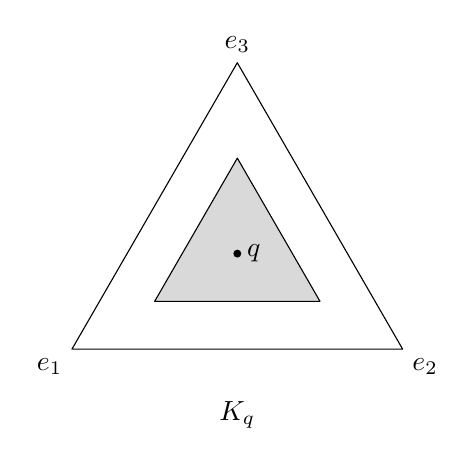
\begin{tikzpicture}[scale=4.2,line join=round]
\coordinate (E1) at (0,0); \coordinate (E2) at (1,0); \coordinate (E3) at (0.5,0.866);
\draw (E1)--(E2)--(E3)--cycle;
\node[below left] at (E1) {$e_1$}; \node[below right] at (E2) {$e_2$}; \node[above] at (E3) {$e_3$};
\fill[gray!30] (0.25,0.1443)--(0.75,0.1443)--(0.5,0.5774)--cycle;
\draw (0.25,0.1443)--(0.75,0.1443)--(0.5,0.5774)--cycle;
\fill (0.5,0.2887) circle (0.012);
\node[right] at (0.5,0.2887) {$q$};
\node at (0.5,-0.2) {$K_q$};
\end{tikzpicture}
\hspace{1.2cm}
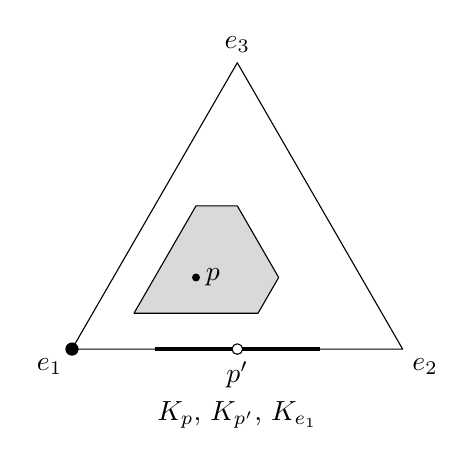
\begin{tikzpicture}[scale=4.2,line join=round]
\coordinate (E1) at (0,0); \coordinate (E2) at (1,0); \coordinate (E3) at (0.5,0.866);
\draw (E1)--(E2)--(E3)--cycle;
\node[below left] at (E1) {$e_1$}; \node[below right] at (E2) {$e_2$}; \node[above] at (E3) {$e_3$};
\fill[gray!30] (0.1875,0.1083)--(0.5625,0.1083)--(0.625,0.2165)--(0.5,0.4330)--(0.375,0.4330)--cycle;
\draw (0.1875,0.1083)--(0.5625,0.1083)--(0.625,0.2165)--(0.5,0.4330)--(0.375,0.4330)--cycle;
\fill (0.375,0.2165) circle (0.012);
\node[right] at (0.375,0.2165) {$p$};
\draw[line width=1.6pt] (0.25,0)--(0.75,0);
\draw[fill=white] (0.5,0) circle (0.016);
\node[below] at (0.5,-0.01) {$p'$};
\fill (E1) circle (0.02);
\node at (0.5,-0.2) {$K_p$, $K_{p'}$, $K_{e_1}$};
\end{tikzpicture}
\caption{Example~\ref{ex:n3}. Left: $K_q$ for $q=(\frac13,\frac13,\frac13)$. Right: $K_p$ for $p=(\frac12,\frac14,\frac14)$ (pentagon), $K_{p'}$ for $p'=(\frac12,\frac12,0)$ (segment), and $K_{e_1}=\{e_1\}$ (point). The point $m\in\Delta$ is drawn at $m_2(1,0)+m_3(\frac12,\frac{\sqrt3}2)$.}
\label{fig:n3}
\end{figure}

\begin{example}\label{ex:n3}
Let $n=3$, $\alpha=\frac12$ and $\beta=2$, so
\[
K_p=\big\{m\in\Delta:\tfrac12p_k\le m_k\le2p_k\ \text{for }k=1,2,3\big\}.
\]
\begin{enumerate}[label=(\roman*)]
\item By Proposition~\ref{prop:band}, $\Ub_p(i)=\min\{2p_i,\frac12(1+p_i)\}$, (U) holds, (Lip) holds with $A=5$, and (Dom) holds with $B=2$. So $\kappa=8\cdot9\cdot9=648$ and $\eta_0=\frac1{1944}$.
\item Let $q:=(\frac13,\frac13,\frac13)$. Then $K_q=\{m\in\Delta:m_k\ge\frac16\text{ for all }k\}$ (the upper bounds $m_k\le\frac23$ follow from the lower bounds), and $K_q=\{\frac12q+\frac12r:r\in\Delta\}$ by Proposition~\ref{prop:band}(iii) with $\varepsilon=\frac12$ (here $1-\varepsilon+\varepsilon/\min_kq_k=2=\beta$). So $K_q$ is the $\varepsilon$-contamination of $q$ with $\varepsilon=\frac12$. Since $\varphi_q(g)=\frac16(g_1+g_2+g_3)+\frac12\min_kg_k$,
\[
D_q=\{g:g_1+g_2+g_3+3\min_kg_k>0\}\cup\{g:g\gneq0\}.
\]
\item $K_{e_1}=\{e_1\}$ and $D_{e_1}=G_1\cup\{g:g\gneq0\}\approx G_1$. For $p':=(\frac12,\frac12,0)$, $K_{p'}=\{m\in\Delta:m_3=0,\ \frac14\le m_1\le\frac34\}$. For $p=(\frac12,\frac14,\frac14)$, $K_p$ is the pentagon with vertices $(\frac34,\frac18,\frac18)$, $(\frac38,\frac12,\frac18)$, $(\frac14,\frac12,\frac14)$, $(\frac14,\frac14,\frac12)$, $(\frac38,\frac18,\frac12)$. See Figure~\ref{fig:n3}.
\item Fix $0<\eta<\frac1{1944}$ and let $L:=L_\eta$. By Theorem~\ref{thm:main}: $L(D_q)=(\frac23,\frac23,\frac23)$ and $D_q$ is undominated; $L(D_{e_1})=(0,1,1)$; and every model $X$ with $X\not\approx D_p$ for all $p\in\Delta$ is dominated by some $D_p$.
\item The model $X:=\{g:g_1+g_2+g_3>0\}\cup\{g:g\gneq0\}$ is coherent (it is $D_K$ with $K:=\{q\}$; Lemma~\ref{lem:basic}(iv)) and has $\Pc_i(X)=\varnothing$ for $i=1,2,3$. So $L(X,\omega_i)\ge2>\frac23=L(D_q,\omega_i)$ for all $i$, and $D_q$ strictly dominates $X$.
\end{enumerate}
\end{example}

\begin{proof}[Proof of (v)]
Fix $i$, let $j,k$ be the other two indices, and suppose $p\in\Pc_i(X)$. The open set $O:=\{g:g_i<0<g_1+g_2+g_3\}$ satisfies $O\subseteq X\setminus G_i\subseteq E_i(X)$, and $E_i(D_p)\setminus G_i=D_p\setminus G_i$. So $\mu(O\setminus D_p)=0$. If $\varphi_p(g^0)<0$ for some $g^0\in O$, then $\{g\in O:\varphi_p(g)<0\}$ is open, nonempty, and disjoint from $D_p$ by Lemma~\ref{lem:basic}(iv), a contradiction. So $m\cdot g\ge0$ for all $m\in K_p$ and $g\in O$. For $\delta>0$ the gambles
\[
-e_i+(1+\delta)e_j,\qquad -\delta e_i+(1+2\delta)e_j-e_k,\qquad -\delta e_i-e_j+(1+2\delta)e_k
\]
lie in $O$. Letting $\delta\to0$ gives $m_j\ge m_i$ and $m_j=m_k$ for all $m\in K_p$. With $m:=p$: $p_j=p_k\ge p_i$, so $p_j=p_k\ge\frac13$. Let $m_i:=p_i$, $m_j:=\frac32p_j$ and $m_k:=\frac12p_k$. Then $m\in K_p$ and $m_j\neq m_k$, a contradiction.
\end{proof}

\begin{thebibliography}{1}
\bibitem{KCM} J.~Konek and C.~Campbell-Moore. Coherence, dominance, and generalized loss. Manuscript.
\end{thebibliography}

\end{document}
